\chapter{Experiments}

\section{Datasets}
\label{sec:datasets}
In the majority of studies that can be found in the literature, the presented models for drug-target interaction prediction are trained and evaluated on binary datasets. Typically, the existing models are evaluated on the four binary datasets that were first presented in \cite{yamanishi2010drug}. In these datasets a label of $y_{d_i, t_j} = 1$ is given for a drug-target pair $(d_i, t_j)$ which is known to interact and a label of $y_{d_i, t_j} = 0$ is given when either the drug-target pair is known not to interact or when it is unknown whether the pair interacts. In contrast to a model that classifies if a drug-target pair interacts or not, the model that is developed in this thesis learns and predicts the continuous binding affinities of drug-target pairs. To the best of my knowledge, only one existing study can be found in the literature which presents a model for the prediction of the continuous binding affinity of drugs and targets, which is the model $KronRLS$ \cite{pahikkala2014toward} which was introduced in section \ref{chp:review}. In the original paper, $KronRLS$ is evaluated on two continuous datasets (\textit{Metz} and \textit{Davis}) that are also used in this thesis for the evaluation of the presented model. A third dataset \textit{KIBA} is obtained by preprocessing the drug-target dataset that is presented in \cite{tang2014making}.
The three datasets named \textit{Metz}, \textit{Davis} and \textit{KIBA} respectively that are used for evaluating the developed model are described in the following chapters. Additionally, the corresponding drug-drug and target-target similarity matrices that were used to construct the graphical model of the CCRF are described in a following section. Table \ref{dataset_stats} lists the sizes and densities of the datasets. Here, density means the percentage of drug-target pairs in the dataset for which an observation is given.

\begin{table}[]
\centering
\begin{tabular}{l c c c}
Dataset & Drugs & Targets & Density \\
\hline
\textit{Davis} & 68 & 442 & 100\%\\
\textit{Metz} & 1421 & 156 & 42.1\%\\
\textit{KIBA} & 2116 & 229 & 24.4\%\\
\end{tabular}
\caption{Statistics of the used evaluation datasets.}
\label{dataset_stats}
\end{table}


\subsection{The Davis Dataset}

The continuous dataset \textit{Davis} was used for the evaluation of the drug-target interaction prediction model presented in \cite{pahikkala2014toward}. The dataset itself was published in the study \cite{davis2011comprehensive}. For this dataset, the interaction of 68 kinase inhibitors with 442 kinases was tested and measured as the $K_d$ value. The kinase inhibitors are the drugs and the kinases are the targets in the more general formulation of drugs and targets. The \textit{Davis} dataset contains the full information of binding affinities for all drug-target pairs in the dataset, and thus contains no missing values. A lower $K_d$ value indicates a higher binding affinity between the drug and the target. As described in \cite{davis2011comprehensive}, the binding affinity is not reported if it was measured to be $>10000$. For these drug target pairs, a $K_d$ value of $10000$ was used for the experiments in this thesis.
The $K_d$ values in the \textit{Davis} dataset were log transformed, according to the formula:

\begin{equation}
pK_d:= -\text{log}_{10}(\frac{K_d}{1e9})
\end{equation}

and thus after the log-transformation a higher $pK_d$ value represents a higher binding affinity. The drug-drug and target-target similarity matrices for this dataset can be downloaded from the website of the author of \cite{pahikkala2014toward}. The distribution of $pK_d$ values in this dataset is illustrated in figure \ref{fig:davis_dist}.

\begin{figure}
\begin{center}
\includegraphics[scale=0.6]{davis_dist.png}
\end{center}
\caption{Distribution of $pK_d$ values given in the \textit{Davis} dataset.}
\label{fig:davis_dist}
\end{figure}

\subsection{The Metz Dataset}

Just as the \textit{Davis} dataset, the continuous dataset \textit{Metz} was used for the evaluation of the drug-target interaction prediction model presented in \cite{pahikkala2014toward}. The dataset was published in the study \cite{metz2011navigating}. The \textit{Metz} dataset consists of 1421 drugs and 156 targets. The binding affinity is given as log transformed $K_i$ values (called $pK_i$ values) for 42$\%$ of the drug-target pairs. As drug-drug and target-target similarities for this dataset the matrices were used that can be downloaded from the website of the author of \cite{pahikkala2014toward}. The distribution of $pK_i$ values in this dataset is illustrated in figure \ref{fig:metz_dist}.
\begin{figure}
\begin{center}
\includegraphics[scale=0.6]{metz_dist.png}
\end{center}
\caption{Distribution of $K_i$ values given in the \textit{Metz} dataset.}
\label{fig:metz_dist}
\end{figure}

\subsection{The KIBA Dataset}

The \textit{Davis} and \textit{Metz} datasets are suitable for the evaluation of predictive models for drug target interaction because data heterogeneity is not an issue. We can assume that the experimental settings for the measured drug target pairs in each dataset were the same and the binding affinities are comparable. When working with experimental results that come from multiple sources the data might be heterogeneous: In one case the binding affinity might be measured by $K_i$, in another case by $K_d$ and in a third case by $IC_{50}$ value. Another source of data heterogeneity are different experimental settings. An approach to integrate the observations from different sources, named \textit{KIBA} (short for \textbf{K}inase \textbf{I}nhibitor \textbf{B}io\textbf{A}ctivity) and a corresponding dataset is presented in \cite{tang2014making}. With their method, the authors of \cite{tang2014making} integrated the experimental results from multiple databases into a bioactivity matrix of 52498 compounds and 467 targets, including 246088 observations. The binding affinities in this matrix are given as \textit{KIBA}-scores. This dataset was used to obtain a third evaluation dataset, which is called the \textit{KIBA} dataset, by removing all drugs and targets with less than 10 observations from the original dataset that was downloaded from the supplementary material of \cite{tang2014making}, resulting in a dataset of 2116 drugs and 229 targets with a density of $~24\%$. For this dataset the drug-drug similarity matrix was computed through the PubChem structure clustering tool (https://pubchem.ncbi.nlm.nih.gov/assay/assay.cgi?p=clustering). The target target similarity matrix was obtained by computing the normalized Smith Waterman Score \cite{yamanishi2010drug} for each pair of targets. The distribution of \textit{KIBA} scores in this dataset is illustrated in figure \ref{fig:kiba_dist}.

\begin{figure}
\begin{center}
\includegraphics[scale=0.6]{kiba_dist.png}
\end{center}
\caption{Distribution of KIBA scores given in the \textit{KIBA} dataset.}
\label{fig:kiba_dist}
\end{figure}

\subsection{Similarity Metrics of Drugs and Targets}
As drug-drug and target-target similarity matrices for the \textit{Davis} and \textit{Metz} dataset the precomputed matrices that are provided on the website of \cite{pahikkala2014toward} were used. Here, the drug-drug similarity was computed based on the 2D chemical structure of the compounds: The compounds are first represented by the graph of their 2D chemical structure and the similarity score is computed based on the size of the common substructures \cite{bajusz2015tanimoto}. The target-target similarity was computed based on the protein sequences, using the normalized Smith-Waterman score \cite{yamanishi2008prediction} . For the \textit{KIBA} dataset, the drug-drug similarity matrix was obtained through the compound clustering tool of PubChem. The given ChEMBL IDs of the compounds were first matched to their PubChem CIDs which were then used as input to the PubChem web interface (The PubChem website offers a tool that allows to match ChEMBL IDs to PubChem CIDs). The clustering tool allows to download a similarity matrix for the compounds which is computed based on the compound structure (similarly as for the drug-drug similarity of the \textit{Metz} and \textit{David} datasets). For the \textit{KIBA} dataset, the protein sequences were downloaded from \textit{NCBI} and the normalized Smith Waterman similarity was computed for each pair by aligning the sequences using the \textit{Biostrings} R package.

\subsubsection{Correlation of Drug/Target Similarity and Binding Behaviour}
In order to examine the correlation between the similarity matrices and the binding behaviour (meaning to find out if similar drugs or targets actually show similar binding behaviour) the following data analysis was performed. First, the analysis regarding the drug-similarity: all pairs of drugs were selected, for which five or more targets can be found, such that both drugs were tested against those five or more targets. The pairs of drugs were subset into two disjunct sets. The first subset contains only pairs of drugs for which the similarity is below a threshold of $0.7$, meaning that this subset contains drug pairs of low similarity. The second subset contains all the drug pairs for which the similarity is above the threshold, meaning this subset contains drug pairs of high similarity. The following steps were then performed for both subsets: For each pair of drugs $(d_a,d_b)$ in the set, all targets that both drugs were tested against were selected. This set of targets was subset into $binding_a$, representing all targets to which $d_a$ binds with a high affinity (the thresholds to define high affinity for the datasets are described in the next section) and $binding_b$, representing all targets to which $d_b$ binds with a high affinity. For each pair of drugs, the size of the union of $binding_a$ and $binding_b$ (x-Axis in the following plots) and the size of the intersection of $binding_a$ and $binding_b$ (y-Axis in the following plot) was computed. Finally, the number of times each combination of union and intersection was obtained is counted (the count is represented by the bubble size and color in the following plots). The same analysis can be repeated analogously for the similar and un-similar target pairs of the datasets.

Figures \ref{fig:metz_drug_simi_corr_1} and \ref{fig:metz_drug_simi_corr_2} show on the x-Axis the size of the union and on the y-Axis the size of the intersection of the drug-drug pairs for the \textit{Metz} dataset. The bubble-size represents the number of drug-drug pairs that were found with the corresponding sizes of the union and intersection. Comparing figures \ref{fig:metz_drug_simi_corr_1} and \ref{fig:metz_drug_simi_corr_2}, we can see that drug-drug pairs with a similarity above $0.7$ tend to share more targets to which both drugs bind with high affinities than drug-drug pairs with a similarity below $0.7$. The same can be observed for drug-drug pairs in the \textit{KIBA} dataset illustrated in figures \ref{fig:kiba_drug_simi_corr_1} and \ref{fig:kiba_drug_simi_corr_2}. For the \textit{Davis} dataset it seems like no such correlation can be observed (see figures \ref{fig:davis_drug_simi_corr_1} and \ref{fig:davis_drug_simi_corr_2}) which goes hand in hand with the observation in the results section, that the drug similarity does not improve the prediction performance. On the other hand as illustrated in figures \ref{fig:davis_target_simi_corr_1} and \ref{fig:davis_target_simi_corr_2}, the target similarity correlates with the binding behaviour of the targets for the \textit{Davis} datasets.


\begin{figure}[p]
\begin{center}
\includegraphics[scale=0.36]{metz_simi_above.png}
\end{center}
\caption[Correlation of drug-similarity and binding behaviour, similar drug pairs, Metz dataset]{Illustration of binding behaviour of drug-drug pairs in \textit{Metz} dataset  with similarity above $0.7$.}
\label{fig:metz_drug_simi_corr_1}
\begin{center}
\includegraphics[scale=0.36]{metz_simi_below.png}
\end{center}
\caption[Correlation of drug-similarity and binding behaviour, un-similar drug pairs, Metz dataset]{Illustration of binding behaviour of drug-drug pairs in \textit{Metz} dataset with similarity below $0.7$.}
\label{fig:metz_drug_simi_corr_2}
\end{figure}


\begin{figure}[p]
\begin{center}
\includegraphics[scale=0.36]{kiba_simi_above.png}
\end{center}
\caption[Correlation of drug-similarity and binding behaviour, similar drug pairs, \textit{KIBA} dataset]{Illustration of binding behaviour of drug-drug pairs in \textit{KIBA} dataset  with similarity above $0.7$.}
\label{fig:kiba_drug_simi_corr_1}
\begin{center}
\includegraphics[scale=0.36]{kiba_simi_below.png}
\end{center}
\caption[Correlation of drug-similarity and binding behaviour, un-similar drug pairs, \textit{KIBA} dataset]{llustration of binding behaviour of drug-drug pairs in \textit{KIBA} dataset  with similarity below $0.7$.}
\label{fig:kiba_drug_simi_corr_2}
\end{figure}

\begin{figure}[p]
\begin{center}
\includegraphics[scale=0.36]{davis_simi_above.png}
\end{center}
\caption[Correlation of drug-similarity and binding behaviour, similar drug pairs, \textit{Davis} dataset]{Illustration of binding behaviour of drug-drug pairs in \textit{Davis} dataset  with similarity above $0.7$.}
\label{fig:davis_drug_simi_corr_1}
\begin{center}
\includegraphics[scale=0.36]{davis_simi_below.png}
\end{center}
\caption[Correlation of drug-similarity and binding behaviour, un-similar drug pairs \textit{Davis} dataset]{Illustration of binding behaviour of drug-drug pairs in \textit{Davis} dataset  with similarity below $0.7$.}
\label{fig:davis_drug_simi_corr_2}
\end{figure}


\begin{figure}[p]
\begin{center}
\includegraphics[scale=0.36]{davis_targets_above.png}
\end{center}
\caption[Correlation of target-similarity and binding behaviour, similar target pairs, \textit{Davis} dataset]{Illustration of binding behaviour of target-target pairs in \textit{Davis} dataset with similarity above $0.7$.}
\label{fig:davis_target_simi_corr_1}
\begin{center}
\includegraphics[scale=0.36]{davis_targets_below.png}
\end{center}
\caption[Correlation of target-similarity and binding behaviour, un-similar target pairs, \textit{Davis} dataset]{Illustration of binding behaviour of target-target pairs in \textit{Davis} dataset with similarity below $0.7$.}
\label{fig:davis_target_simi_corr_2}
\end{figure}







\section{Experimental Settings}

\subsection{Integrating the similarity matrices}
For the MF+CCRF method that is developed in this thesis it is possible to integrate:
\begin{itemize}
\item none of the similarity matrices
\item only the drug drug similarity matrix
\item only the target target similarity matrix
\item both similarity matrices
\end{itemize}
Here, using no similarity metric means to use just the MF prediction. When only the drug-drug similarity metric is used, we build graphical models for each column of the matrix. Thus a separate set of parameters is learned and independent predictions are made for each target. Similarly, if only the target-target similarity metric is used, a separate graphical model is build for each row of the matrix and separate paratemers are learned and independant predictions made for each drug. When both similarity matrices are used each cell of the matrix becomes a node of the CCRF and by default we would learn only one set of parameters for this CCRF. The datasets that were used for the experiments in this thesis are too large to create a single graphical model for all drugs and targets because in the inference step it is necessary to compute the inverse of a matrix of size $|D||T| \times |D||T|$. In order to integrate both similarity matrices for the CCRF the drug-target matrix was clustered into smaller submatrices of feasible size. 


\begin{figure}
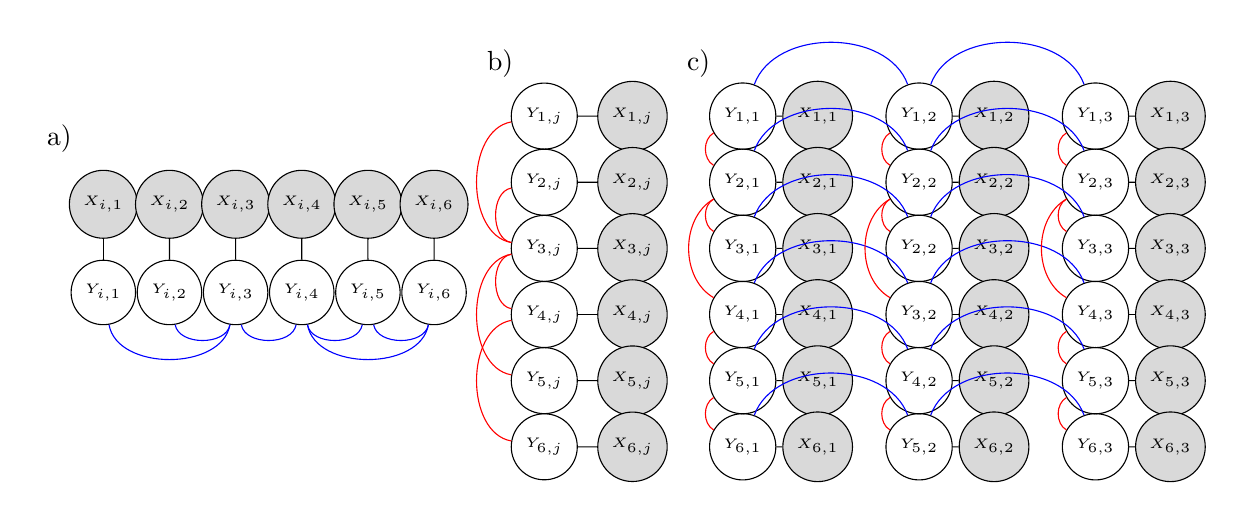
\begin{tikzpicture}[scale=0.56]
\tikzstyle{every node} = [draw, shape=circle]
\node[draw=none] (a) at (-1, 3.5) {a)};
\node (a) at (0, 0) {\tiny $Y_{i, 1}$};
\node (b) at (1.5, 0) {\tiny $Y_{i, 2}$};
\node (c) at (3, 0) {\tiny $Y_{i, 3}$};
\node (d) at (4.5, 0) {\tiny $Y_{i, 4}$};
\node (e) at (6, 0) {\tiny $Y_{i, 5}$};
\node (f) at (7.5, 0) {\tiny $Y_{i, 6}$};
\draw [-, draw=blue] (a) to  [out=280,in=260] (c);
\draw [-, draw=blue] (b) to  [out=280,in=260] (c);
\draw [-, draw=blue] (e) to  [out=280,in=260] (f);
\draw [-, draw=blue] (c) to  [out=280,in=260] (d);
\draw [-, draw=blue] (d) to  [out=280,in=260] (e);
\draw [-, draw=blue] (d) to  [out=280,in=260] (f);

\node [fill=gray!30](ax) at (0, 2) {\tiny $X_{i, 1}$};
\node [fill=gray!30](bx) at (1.5, 2) {\tiny $X_{i, 2}$};
\node [fill=gray!30](cx) at (3, 2) {\tiny $X_{i, 3}$};
\node [fill=gray!30](dx) at (4.5, 2) {\tiny $X_{i, 4}$};
\node [fill=gray!30](ex) at (6, 2) {\tiny $X_{i, 5}$};
\node [fill=gray!30](fx) at (7.5, 2) {\tiny $X_{i, 6}$};

\draw [-] (a) to  [out=90,in=270] (ax);
\draw [-] (b) to  [out=90,in=270] (bx);
\draw [-] (c) to  [out=90,in=270] (cx);
\draw [-] (d) to  [out=90,in=270] (dx);
\draw [-] (e) to  [out=90,in=270] (ex);
\draw [-] (f) to  [out=90,in=270] (fx);

\node[draw=none] (a) at (9, 5.2) {b)};
\node (a) at (10, 4) {\tiny $Y_{1,j}$};
\node (b) at (10, 2.5) {\tiny $Y_{2,j}$};
\node (c) at (10, 1) {\tiny $Y_{3,j}$};
\node (d) at (10, -0.5) {\tiny $Y_{4,j}$};
\node (e) at (10, -2) {\tiny $Y_{5,j}$};
\node (f) at (10, -3.5) {\tiny $Y_{6,j}$};

\node [fill=gray!30](ax) at (12, 4) {\tiny $X_{1,j}$};
\node [fill=gray!30](bx) at (12, 2.5) {\tiny $X_{2,j}$};
\node [fill=gray!30](cx) at (12, 1) {\tiny $X_{3,j}$};
\node [fill=gray!30](dx) at (12, -0.5) {\tiny $X_{4,j}$};
\node [fill=gray!30](ex) at (12, -2) {\tiny $X_{5,j}$};
\node [fill=gray!30](fx) at (12, -3.5) {\tiny $X_{6,j}$};

\draw [-] (a) to  [out=0,in=180] (ax);
\draw [-] (b) to  [out=0,in=180] (bx);
\draw [-] (c) to  [out=0,in=180] (cx);
\draw [-] (d) to  [out=0,in=180] (dx);
\draw [-] (e) to  [out=0,in=180] (ex);
\draw [-] (f) to  [out=0,in=180] (fx);

\draw [-, draw=red] (a) to  [out=190,in=170] (c);
\draw [-, draw=red] (c) to  [out=190,in=170] (d);
\draw [-, draw=red] (d) to  [out=190,in=170] (f);
\draw [-, draw=red] (b) to  [out=190,in=170] (c);
\draw [-, draw=red] (c) to  [out=190,in=170] (e);

\node[draw=none] (a) at (13.5, 5.2) {c)};
\node (a) at (14.5, 4) {\tiny $Y_{1,1}$};
\node (b) at (14.5, 2.5) {\tiny $Y_{2, 1}$};
\node (c) at (14.5, 1) {\tiny $Y_{3,1}$};
\node (d) at (14.5, -0.5) {\tiny $Y_{4, 1}$};
\node (e) at (14.5, -2) {\tiny $Y_{5, 1}$};
\node (f) at (14.5, -3.5) {\tiny $Y_{6, 1}$};

\node [fill=gray!30](ax) at (16.2, 4) {\tiny $X_{1, 1}$};
\node [fill=gray!30](bx) at (16.2, 2.5) {\tiny $X_{2, 1}$};
\node [fill=gray!30](cx) at (16.2, 1) {\tiny $X_{3, 1}$};
\node [fill=gray!30](dx) at (16.2, -0.5) {\tiny $X_{4, 1}$};
\node [fill=gray!30](ex) at (16.2, -2) {\tiny $X_{5, 1}$};
\node [fill=gray!30](fx) at (16.2, -3.5) {\tiny $X_{6, 1}$};


\draw [-] (a) to  [out=0,in=180] (ax);
\draw [-] (b) to  [out=0,in=180] (bx);
\draw [-] (c) to  [out=0,in=180] (cx);
\draw [-] (d) to  [out=0,in=180] (dx);
\draw [-] (e) to  [out=0,in=180] (ex);
\draw [-] (f) to  [out=0,in=180] (fx);

\node (a_) at (18.5, 4) {\tiny $Y_{1,2}$};
\node (b_) at (18.5, 2.5) {\tiny $Y_{2,2}$};
\node (c_) at (18.5, 1) {\tiny $Y_{2,2}$};
\node (d_) at (18.5, -0.5) {\tiny $Y_{3,2}$};
\node (e_) at (18.5, -2) {\tiny $Y_{4,2}$};
\node (f_) at (18.5, -3.5) {\tiny $Y_{5,2}$};

\node[fill=gray!30] (ax_) at (20.2, 4) {\tiny $X_{1,2}$};
\node[fill=gray!30] (bx_) at (20.2, 2.5) {\tiny $X_{2,2}$};
\node[fill=gray!30] (cx_) at (20.2, 1) {\tiny $X_{3,2}$};
\node[fill=gray!30] (dx_) at (20.2, -0.5) {\tiny $X_{4,2}$};
\node[fill=gray!30] (ex_) at (20.2, -2) {\tiny $X_{5,2}$};
\node[fill=gray!30] (fx_) at (20.2, -3.5) {\tiny $X_{6,2}$};

\draw [-] (a_) to  [out=0,in=180] (ax_);
\draw [-] (b_) to  [out=0,in=180] (bx_);
\draw [-] (c_) to  [out=0,in=180] (cx_);
\draw [-] (d_) to  [out=0,in=180] (dx_);
\draw [-] (e_) to  [out=0,in=180] (ex_);
\draw [-] (f_) to  [out=0,in=180] (fx_);

\node (a__) at (22.5, 4) {\tiny $Y_{1,3}$};
\node (b__) at (22.5, 2.5) {\tiny $Y_{2,3}$};
\node (c__) at (22.5, 1) {\tiny $Y_{3,3}$};
\node (d__) at (22.5, -0.5) {\tiny $Y_{4,3}$};
\node (e__) at (22.5, -2) {\tiny $Y_{5,3}$};
\node (f__) at (22.5, -3.5) {\tiny $Y_{6,3}$};

\node[fill=gray!30] (ax__) at (24.2, 4) {\tiny $X_{1, 3}$};
\node[fill=gray!30] (bx__) at (24.2, 2.5) {\tiny $X_{2, 3}$};
\node[fill=gray!30] (cx__) at (24.2, 1) {\tiny $X_{3, 3}$};
\node[fill=gray!30] (dx__) at (24.2, -0.5) {\tiny $X_{4, 3}$};
\node[fill=gray!30] (ex__) at (24.2, -2) {\tiny $X_{5, 3}$};
\node[fill=gray!30] (fx__) at (24.2, -3.5) {\tiny $X_{6,3}$};

\draw [-] (a__) to  [out=0,in=180] (ax__);
\draw [-] (b__) to  [out=0,in=180] (bx__);
\draw [-] (c__) to  [out=0,in=180] (cx__);
\draw [-] (d__) to  [out=0,in=180] (dx__);
\draw [-] (e__) to  [out=0,in=180] (ex__);
\draw [-] (f__) to  [out=0,in=180] (fx__);

\draw [-, draw=blue] (a) to  [out=70,in=110] (a_);
\draw [-, draw=blue] (a_) to  [out=70,in=110] (a__);
\draw [-, draw=blue] (b) to  [out=70,in=110] (b_);
\draw [-, draw=blue] (b_) to  [out=70,in=110] (b__);
\draw [-, draw=blue] (c) to  [out=70,in=110] (c_);
\draw [-, draw=blue] (c_) to  [out=70,in=110] (c__);
\draw [-, draw=blue] (d) to  [out=70,in=110] (d_);
\draw [-, draw=blue] (d_) to  [out=70,in=110] (d__);
\draw [-, draw=blue] (e) to  [out=70,in=110] (e_);
\draw [-, draw=blue] (e_) to  [out=70,in=110] (e__);
\draw [-, draw=blue] (f) to  [out=70,in=110] (f_);
\draw [-, draw=blue] (f_) to  [out=70,in=110] (f__);


\draw [-, draw=red] (a) to  [out=210,in=150] (b);
\draw [-, draw=red] (b) to  [out=210,in=150] (c);
\draw [-, draw=red] (b) to  [out=210,in=150] (d);
\draw [-, draw=red] (d) to  [out=210,in=150] (e);
\draw [-, draw=red] (e) to  [out=210,in=150] (f);

\draw [-, draw=red] (a_) to  [out=210,in=150] (b_);
\draw [-, draw=red] (b_) to  [out=210,in=150] (c_);
\draw [-, draw=red] (b_) to  [out=210,in=150] (d_);
\draw [-, draw=red] (d_) to  [out=210,in=150] (e_);
\draw [-, draw=red] (e_) to  [out=210,in=150] (f_);

\draw [-, draw=red] (a__) to  [out=210,in=150] (b__);
\draw [-, draw=red] (b__) to  [out=210,in=150] (c__);
\draw [-, draw=red] (b__) to  [out=210,in=150] (d__);
\draw [-, draw=red] (d__) to  [out=210,in=150] (e__);
\draw [-, draw=red] (e__) to  [out=210,in=150] (f__);
\end{tikzpicture}
\caption[Integrating similarity matrices]{Integrating the similarity matrices: a) integration of only the target similarity matrix. The cells $Y_{i,1},\dots,Y_{i,6}$ indicate the predictions that are to be made for drug $d_i$. $X_{i,1},\dots, X_{i,6}$ indicate the predictions made by Matrix Factorization for those targets. Blue edges indicate similar targets. b) integration of only the drug similarity matrix. The cells $Y_{1,j},\dots,Y_{6,j}$ indicate the predictions that are to be made for target $t_j$. Red edges indicate similar drugs. c) integration of both similarity matrices. The cells $Y_{i,j}$ indicate the predictions that are to be made for the drug-target pairs in the cluster, consisting of drugs $d_1,d_2,d_3$ and targets $t_1,\dots,t_6$.}
\end{figure}

\subsection{Parallelization}


\subsection{Graphical structure of CCRF}

As mentioned in \ref{sec:MFCCRF}, different strategies can be applied to chose the edges of the graphical model. Which of the CCRF nodes are connected is defined through the similarity matrix $S$ in the formulation of the CCRF. Theoretically, one can connect all nodes to all other nodes and weight the edges with the similarity between the corresponding drugs or targets. However, the time of computing the covariance matrix of the Gaussian distribution, which is defined through the CCRF depends on the sparsity of $S$. It is necessary to compute this inverse in each step of the parameter learning as well as in the inference step. In order to get CCRFs with a feasible structure, the edges for the experiments in this thesis where chosen by connecting all drugs and targets to its $k=4$ nearest neighbors. An other strategy to connect the nodes, that was tested in this thesis is to chose a similarity-threshold $t$ and connect all drugs and targets with a similarity above the threshold.



